% Created by tikzDevice version 0.12.3.1 on 2021-12-08 19:12:01
% !TEX encoding = UTF-8 Unicode
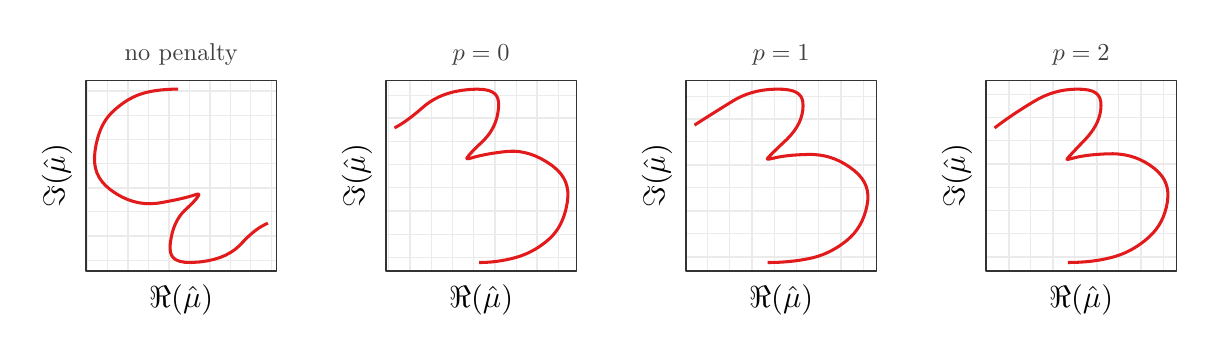
\begin{tikzpicture}[x=1pt,y=1pt]
\definecolor{fillColor}{RGB}{255,255,255}
\begin{scope}
\definecolor{drawColor}{RGB}{255,255,255}
\definecolor{fillColor}{RGB}{255,255,255}

\path[draw=drawColor,line width= 0.6pt,line join=round,line cap=round,fill=fillColor] (  6.64,  0.00) rectangle (101.77,108.41);
\end{scope}
\begin{scope}
\definecolor{fillColor}{RGB}{255,255,255}

\path[fill=fillColor] ( 27.35, 20.71) rectangle ( 96.27, 89.63);
\definecolor{drawColor}{gray}{0.92}

\path[draw=drawColor,line width= 0.3pt,line join=round] ( 27.35, 24.73) --
	( 96.27, 24.73);

\path[draw=drawColor,line width= 0.3pt,line join=round] ( 27.35, 42.16) --
	( 96.27, 42.16);

\path[draw=drawColor,line width= 0.3pt,line join=round] ( 27.35, 59.59) --
	( 96.27, 59.59);

\path[draw=drawColor,line width= 0.3pt,line join=round] ( 27.35, 77.02) --
	( 96.27, 77.02);

\path[draw=drawColor,line width= 0.3pt,line join=round] ( 35.32, 20.71) --
	( 35.32, 89.63);

\path[draw=drawColor,line width= 0.3pt,line join=round] ( 50.05, 20.71) --
	( 50.05, 89.63);

\path[draw=drawColor,line width= 0.3pt,line join=round] ( 64.79, 20.71) --
	( 64.79, 89.63);

\path[draw=drawColor,line width= 0.3pt,line join=round] ( 79.52, 20.71) --
	( 79.52, 89.63);

\path[draw=drawColor,line width= 0.3pt,line join=round] ( 94.25, 20.71) --
	( 94.25, 89.63);

\path[draw=drawColor,line width= 0.6pt,line join=round] ( 27.35, 33.44) --
	( 96.27, 33.44);

\path[draw=drawColor,line width= 0.6pt,line join=round] ( 27.35, 50.87) --
	( 96.27, 50.87);

\path[draw=drawColor,line width= 0.6pt,line join=round] ( 27.35, 68.30) --
	( 96.27, 68.30);

\path[draw=drawColor,line width= 0.6pt,line join=round] ( 27.35, 85.73) --
	( 96.27, 85.73);

\path[draw=drawColor,line width= 0.6pt,line join=round] ( 27.96, 20.71) --
	( 27.96, 89.63);

\path[draw=drawColor,line width= 0.6pt,line join=round] ( 42.69, 20.71) --
	( 42.69, 89.63);

\path[draw=drawColor,line width= 0.6pt,line join=round] ( 57.42, 20.71) --
	( 57.42, 89.63);

\path[draw=drawColor,line width= 0.6pt,line join=round] ( 72.15, 20.71) --
	( 72.15, 89.63);

\path[draw=drawColor,line width= 0.6pt,line join=round] ( 86.88, 20.71) --
	( 86.88, 89.63);
\definecolor{drawColor}{RGB}{227,26,28}

\path[draw=drawColor,line width= 1.1pt,line join=round] ( 60.67, 86.50) --
	( 58.45, 86.47) --
	( 56.39, 86.36) --
	( 54.48, 86.20) --
	( 52.71, 85.98) --
	( 51.08, 85.71) --
	( 49.58, 85.39) --
	( 48.21, 85.03) --
	( 46.94, 84.63) --
	( 45.76, 84.18) --
	( 44.60, 83.66) --
	( 43.45, 83.07) --
	( 42.29, 82.41) --
	( 41.14, 81.66) --
	( 40.00, 80.84) --
	( 38.85, 79.93) --
	( 37.69, 78.93) --
	( 36.54, 77.84) --
	( 35.48, 76.65) --
	( 34.52, 75.35) --
	( 33.65, 73.91) --
	( 32.88, 72.34) --
	( 32.19, 70.60) --
	( 31.60, 68.69) --
	( 31.09, 66.58) --
	( 30.69, 64.24) --
	( 30.48, 61.93) --
	( 30.54, 59.87) --
	( 30.83, 58.01) --
	( 31.35, 56.30) --
	( 32.12, 54.69) --
	( 33.16, 53.14) --
	( 34.52, 51.63) --
	( 36.25, 50.14) --
	( 38.30, 48.73) --
	( 40.37, 47.56) --
	( 42.42, 46.63) --
	( 44.47, 45.93) --
	( 46.54, 45.44) --
	( 48.63, 45.16) --
	( 50.78, 45.09) --
	( 52.98, 45.24) --
	( 55.25, 45.60) --
	( 57.35, 46.00) --
	( 59.23, 46.37) --
	( 60.91, 46.73) --
	( 62.38, 47.07) --
	( 63.68, 47.40) --
	( 64.80, 47.70) --
	( 65.76, 47.98) --
	( 66.58, 48.24) --
	( 67.21, 48.44) --
	( 67.64, 48.53) --
	( 67.91, 48.56) --
	( 68.06, 48.54) --
	( 68.14, 48.49) --
	( 68.17, 48.43) --
	( 68.16, 48.33) --
	( 68.10, 48.16) --
	( 67.97, 47.89) --
	( 67.76, 47.55) --
	( 67.47, 47.14) --
	( 67.08, 46.65) --
	( 66.57, 46.08) --
	( 65.94, 45.40) --
	( 65.16, 44.63) --
	( 64.23, 43.74) --
	( 63.14, 42.73) --
	( 62.11, 41.64) --
	( 61.20, 40.46) --
	( 60.40, 39.17) --
	( 59.70, 37.78) --
	( 59.09, 36.26) --
	( 58.58, 34.59) --
	( 58.18, 32.75) --
	( 57.87, 30.73) --
	( 57.78, 28.87) --
	( 57.97, 27.47) --
	( 58.36, 26.40) --
	( 58.99, 25.55) --
	( 59.90, 24.85) --
	( 61.20, 24.31) --
	( 63.03, 23.95) --
	( 65.52, 23.85) --
	( 68.54, 24.05) --
	( 71.30, 24.45) --
	( 73.78, 25.01) --
	( 76.00, 25.72) --
	( 77.99, 26.56) --
	( 79.77, 27.54) --
	( 81.36, 28.64) --
	( 82.79, 29.88) --
	( 84.08, 31.24) --
	( 85.32, 32.52) --
	( 86.52, 33.66) --
	( 87.69, 34.67) --
	( 88.83, 35.56) --
	( 89.94, 36.34) --
	( 91.03, 37.01) --
	( 92.09, 37.58) --
	( 93.14, 38.06);
\definecolor{drawColor}{gray}{0.20}

\path[draw=drawColor,line width= 0.6pt,line join=round,line cap=round] ( 27.35, 20.71) rectangle ( 96.27, 89.63);
\end{scope}
\begin{scope}
\definecolor{drawColor}{RGB}{0,0,0}

\node[text=drawColor,anchor=base,inner sep=0pt, outer sep=0pt, scale=  1.10] at ( 61.81,  7.64) {$\Re(\hat\mu)$};
\end{scope}
\begin{scope}
\definecolor{drawColor}{RGB}{0,0,0}

\node[text=drawColor,rotate= 90.00,anchor=base,inner sep=0pt, outer sep=0pt, scale=  1.10] at ( 19.71, 55.17) {$\Im(\hat\mu)$};
\end{scope}
\begin{scope}
\definecolor{drawColor}{gray}{0.25}

\node[text=drawColor,anchor=base,inner sep=0pt, outer sep=0pt, scale=  0.88] at ( 61.81, 96.84) {no penalty};
\end{scope}
\begin{scope}
\definecolor{drawColor}{RGB}{255,255,255}
\definecolor{fillColor}{RGB}{255,255,255}

\path[draw=drawColor,line width= 0.6pt,line join=round,line cap=round,fill=fillColor] (115.04,  0.00) rectangle (210.17,108.41);
\end{scope}
\begin{scope}
\definecolor{fillColor}{RGB}{255,255,255}

\path[fill=fillColor] (135.76, 20.71) rectangle (204.67, 89.63);
\definecolor{drawColor}{gray}{0.92}

\path[draw=drawColor,line width= 0.3pt,line join=round] (135.76, 34.03) --
	(204.67, 34.03);

\path[draw=drawColor,line width= 0.3pt,line join=round] (135.76, 50.83) --
	(204.67, 50.83);

\path[draw=drawColor,line width= 0.3pt,line join=round] (135.76, 67.62) --
	(204.67, 67.62);

\path[draw=drawColor,line width= 0.3pt,line join=round] (135.76, 84.41) --
	(204.67, 84.41);

\path[draw=drawColor,line width= 0.3pt,line join=round] (136.86, 20.71) --
	(136.86, 89.63);

\path[draw=drawColor,line width= 0.3pt,line join=round] (152.16, 20.71) --
	(152.16, 89.63);

\path[draw=drawColor,line width= 0.3pt,line join=round] (167.47, 20.71) --
	(167.47, 89.63);

\path[draw=drawColor,line width= 0.3pt,line join=round] (182.77, 20.71) --
	(182.77, 89.63);

\path[draw=drawColor,line width= 0.3pt,line join=round] (198.08, 20.71) --
	(198.08, 89.63);

\path[draw=drawColor,line width= 0.6pt,line join=round] (135.76, 25.64) --
	(204.67, 25.64);

\path[draw=drawColor,line width= 0.6pt,line join=round] (135.76, 42.43) --
	(204.67, 42.43);

\path[draw=drawColor,line width= 0.6pt,line join=round] (135.76, 59.22) --
	(204.67, 59.22);

\path[draw=drawColor,line width= 0.6pt,line join=round] (135.76, 76.01) --
	(204.67, 76.01);

\path[draw=drawColor,line width= 0.6pt,line join=round] (144.51, 20.71) --
	(144.51, 89.63);

\path[draw=drawColor,line width= 0.6pt,line join=round] (159.82, 20.71) --
	(159.82, 89.63);

\path[draw=drawColor,line width= 0.6pt,line join=round] (175.12, 20.71) --
	(175.12, 89.63);

\path[draw=drawColor,line width= 0.6pt,line join=round] (190.42, 20.71) --
	(190.42, 89.63);
\definecolor{drawColor}{RGB}{227,26,28}

\path[draw=drawColor,line width= 1.1pt,line join=round] (169.47, 23.85) --
	(171.04, 23.87) --
	(172.61, 23.95) --
	(174.18, 24.07) --
	(175.74, 24.25) --
	(177.30, 24.48) --
	(178.87, 24.76) --
	(180.43, 25.09) --
	(182.01, 25.48) --
	(183.57, 25.92) --
	(185.09, 26.44) --
	(186.58, 27.04) --
	(188.02, 27.72) --
	(189.44, 28.48) --
	(190.83, 29.32) --
	(192.19, 30.26) --
	(193.53, 31.28) --
	(194.84, 32.39) --
	(196.05, 33.60) --
	(197.12, 34.90) --
	(198.09, 36.31) --
	(198.94, 37.83) --
	(199.69, 39.49) --
	(200.34, 41.31) --
	(200.88, 43.29) --
	(201.31, 45.47) --
	(201.54, 47.62) --
	(201.51, 49.55) --
	(201.23, 51.29) --
	(200.73, 52.91) --
	(199.98, 54.45) --
	(198.96, 55.93) --
	(197.62, 57.39) --
	(195.92, 58.83) --
	(193.89, 60.21) --
	(191.88, 61.36) --
	(189.92, 62.29) --
	(187.97, 63.02) --
	(186.04, 63.55) --
	(184.11, 63.90) --
	(182.17, 64.06) --
	(180.21, 64.04) --
	(178.21, 63.85) --
	(176.32, 63.60) --
	(174.59, 63.35) --
	(173.00, 63.09) --
	(171.55, 62.82) --
	(170.24, 62.55) --
	(169.04, 62.27) --
	(167.97, 62.00) --
	(167.01, 61.72) --
	(166.23, 61.50) --
	(165.70, 61.39) --
	(165.37, 61.35) --
	(165.18, 61.36) --
	(165.09, 61.39) --
	(165.06, 61.44) --
	(165.06, 61.52) --
	(165.11, 61.66) --
	(165.25, 61.89) --
	(165.48, 62.21) --
	(165.80, 62.62) --
	(166.25, 63.14) --
	(166.84, 63.78) --
	(167.59, 64.56) --
	(168.52, 65.50) --
	(169.66, 66.59) --
	(170.98, 67.85) --
	(172.21, 69.18) --
	(173.26, 70.54) --
	(174.15, 71.94) --
	(174.89, 73.40) --
	(175.50, 74.93) --
	(175.97, 76.54) --
	(176.31, 78.26) --
	(176.51, 80.09) --
	(176.50, 81.76) --
	(176.25, 83.03) --
	(175.80, 84.03) --
	(175.12, 84.84) --
	(174.17, 85.50) --
	(172.84, 86.03) --
	(171.01, 86.38) --
	(168.57, 86.50) --
	(165.62, 86.35) --
	(162.86, 86.02) --
	(160.32, 85.53) --
	(157.99, 84.88) --
	(155.83, 84.09) --
	(153.83, 83.15) --
	(151.98, 82.07) --
	(150.25, 80.84) --
	(148.64, 79.48) --
	(147.13, 78.19) --
	(145.70, 77.04) --
	(144.37, 76.01) --
	(143.11, 75.09) --
	(141.95, 74.30) --
	(140.85, 73.60) --
	(139.84, 73.00) --
	(138.89, 72.50);
\definecolor{drawColor}{gray}{0.20}

\path[draw=drawColor,line width= 0.6pt,line join=round,line cap=round] (135.76, 20.71) rectangle (204.67, 89.63);
\end{scope}
\begin{scope}
\definecolor{drawColor}{RGB}{0,0,0}

\node[text=drawColor,anchor=base,inner sep=0pt, outer sep=0pt, scale=  1.10] at (170.21,  7.64) {$\Re(\hat\mu)$};
\end{scope}
\begin{scope}
\definecolor{drawColor}{RGB}{0,0,0}

\node[text=drawColor,rotate= 90.00,anchor=base,inner sep=0pt, outer sep=0pt, scale=  1.10] at (128.12, 55.17) {$\Im(\hat\mu)$};
\end{scope}
\begin{scope}
\definecolor{drawColor}{gray}{0.25}

\node[text=drawColor,anchor=base,inner sep=0pt, outer sep=0pt, scale=  0.88] at (170.21, 96.84) {$p = 0$};
\end{scope}
\begin{scope}
\definecolor{drawColor}{RGB}{255,255,255}
\definecolor{fillColor}{RGB}{255,255,255}

\path[draw=drawColor,line width= 0.6pt,line join=round,line cap=round,fill=fillColor] (223.45,  0.00) rectangle (318.58,108.41);
\end{scope}
\begin{scope}
\definecolor{fillColor}{RGB}{255,255,255}

\path[fill=fillColor] (244.16, 20.71) rectangle (313.08, 89.63);
\definecolor{drawColor}{gray}{0.92}

\path[draw=drawColor,line width= 0.3pt,line join=round] (244.16, 34.24) --
	(313.08, 34.24);

\path[draw=drawColor,line width= 0.3pt,line join=round] (244.16, 50.84) --
	(313.08, 50.84);

\path[draw=drawColor,line width= 0.3pt,line join=round] (244.16, 67.43) --
	(313.08, 67.43);

\path[draw=drawColor,line width= 0.3pt,line join=round] (244.16, 84.03) --
	(313.08, 84.03);

\path[draw=drawColor,line width= 0.3pt,line join=round] (260.08, 20.71) --
	(260.08, 89.63);

\path[draw=drawColor,line width= 0.3pt,line join=round] (276.12, 20.71) --
	(276.12, 89.63);

\path[draw=drawColor,line width= 0.3pt,line join=round] (292.17, 20.71) --
	(292.17, 89.63);

\path[draw=drawColor,line width= 0.3pt,line join=round] (308.21, 20.71) --
	(308.21, 89.63);

\path[draw=drawColor,line width= 0.6pt,line join=round] (244.16, 25.94) --
	(313.08, 25.94);

\path[draw=drawColor,line width= 0.6pt,line join=round] (244.16, 42.54) --
	(313.08, 42.54);

\path[draw=drawColor,line width= 0.6pt,line join=round] (244.16, 59.13) --
	(313.08, 59.13);

\path[draw=drawColor,line width= 0.6pt,line join=round] (244.16, 75.73) --
	(313.08, 75.73);

\path[draw=drawColor,line width= 0.6pt,line join=round] (252.05, 20.71) --
	(252.05, 89.63);

\path[draw=drawColor,line width= 0.6pt,line join=round] (268.10, 20.71) --
	(268.10, 89.63);

\path[draw=drawColor,line width= 0.6pt,line join=round] (284.15, 20.71) --
	(284.15, 89.63);

\path[draw=drawColor,line width= 0.6pt,line join=round] (300.19, 20.71) --
	(300.19, 89.63);
\definecolor{drawColor}{RGB}{227,26,28}

\path[draw=drawColor,line width= 1.1pt,line join=round] (273.73, 23.85) --
	(275.79, 23.87) --
	(277.79, 23.94) --
	(279.73, 24.06) --
	(281.62, 24.22) --
	(283.46, 24.42) --
	(285.25, 24.66) --
	(286.98, 24.95) --
	(288.67, 25.27) --
	(290.32, 25.65) --
	(291.93, 26.11) --
	(293.50, 26.66) --
	(295.05, 27.30) --
	(296.57, 28.03) --
	(298.08, 28.86) --
	(299.57, 29.79) --
	(301.04, 30.82) --
	(302.50, 31.96) --
	(303.84, 33.18) --
	(305.03, 34.47) --
	(306.09, 35.85) --
	(307.03, 37.32) --
	(307.85, 38.90) --
	(308.55, 40.60) --
	(309.15, 42.44) --
	(309.63, 44.43) --
	(309.91, 46.39) --
	(309.95, 48.17) --
	(309.75, 49.80) --
	(309.33, 51.33) --
	(308.69, 52.78) --
	(307.80, 54.20) --
	(306.62, 55.60) --
	(305.12, 57.00) --
	(303.33, 58.35) --
	(301.51, 59.52) --
	(299.68, 60.50) --
	(297.84, 61.30) --
	(295.97, 61.94) --
	(294.05, 62.42) --
	(292.09, 62.73) --
	(290.05, 62.89) --
	(287.95, 62.89) --
	(285.95, 62.82) --
	(284.10, 62.72) --
	(282.40, 62.59) --
	(280.83, 62.43) --
	(279.40, 62.24) --
	(278.09, 62.03) --
	(276.91, 61.80) --
	(275.83, 61.55) --
	(274.96, 61.35) --
	(274.36, 61.24) --
	(273.97, 61.20) --
	(273.76, 61.20) --
	(273.66, 61.23) --
	(273.62, 61.27) --
	(273.62, 61.32) --
	(273.67, 61.43) --
	(273.81, 61.61) --
	(274.05, 61.89) --
	(274.41, 62.29) --
	(274.92, 62.82) --
	(275.61, 63.52) --
	(276.50, 64.40) --
	(277.62, 65.48) --
	(278.99, 66.78) --
	(280.62, 68.31) --
	(282.09, 69.87) --
	(283.31, 71.39) --
	(284.31, 72.88) --
	(285.10, 74.36) --
	(285.71, 75.84) --
	(286.14, 77.33) --
	(286.41, 78.85) --
	(286.52, 80.42) --
	(286.44, 81.84) --
	(286.16, 82.97) --
	(285.70, 83.88) --
	(285.05, 84.64) --
	(284.16, 85.28) --
	(282.97, 85.81) --
	(281.39, 86.21) --
	(279.32, 86.45) --
	(276.85, 86.50) --
	(274.46, 86.40) --
	(272.20, 86.15) --
	(270.05, 85.76) --
	(267.99, 85.24) --
	(266.01, 84.59) --
	(264.11, 83.80) --
	(262.28, 82.87) --
	(260.50, 81.81) --
	(258.75, 80.73) --
	(257.03, 79.66) --
	(255.33, 78.60) --
	(253.67, 77.56) --
	(252.04, 76.53) --
	(250.43, 75.51) --
	(248.85, 74.50) --
	(247.29, 73.50);
\definecolor{drawColor}{gray}{0.20}

\path[draw=drawColor,line width= 0.6pt,line join=round,line cap=round] (244.16, 20.71) rectangle (313.08, 89.63);
\end{scope}
\begin{scope}
\definecolor{drawColor}{RGB}{0,0,0}

\node[text=drawColor,anchor=base,inner sep=0pt, outer sep=0pt, scale=  1.10] at (278.62,  7.64) {$\Re(\hat\mu)$};
\end{scope}
\begin{scope}
\definecolor{drawColor}{RGB}{0,0,0}

\node[text=drawColor,rotate= 90.00,anchor=base,inner sep=0pt, outer sep=0pt, scale=  1.10] at (236.52, 55.17) {$\Im(\hat\mu)$};
\end{scope}
\begin{scope}
\definecolor{drawColor}{gray}{0.25}

\node[text=drawColor,anchor=base,inner sep=0pt, outer sep=0pt, scale=  0.88] at (278.62, 96.84) {$p = 1$};
\end{scope}
\begin{scope}
\definecolor{drawColor}{RGB}{255,255,255}
\definecolor{fillColor}{RGB}{255,255,255}

\path[draw=drawColor,line width= 0.6pt,line join=round,line cap=round,fill=fillColor] (331.85,  0.00) rectangle (426.98,108.41);
\end{scope}
\begin{scope}
\definecolor{fillColor}{RGB}{255,255,255}

\path[fill=fillColor] (352.57, 20.71) rectangle (421.48, 89.63);
\definecolor{drawColor}{gray}{0.92}

\path[draw=drawColor,line width= 0.3pt,line join=round] (352.57, 34.32) --
	(421.48, 34.32);

\path[draw=drawColor,line width= 0.3pt,line join=round] (352.57, 51.08) --
	(421.48, 51.08);

\path[draw=drawColor,line width= 0.3pt,line join=round] (352.57, 67.83) --
	(421.48, 67.83);

\path[draw=drawColor,line width= 0.3pt,line join=round] (352.57, 84.59) --
	(421.48, 84.59);

\path[draw=drawColor,line width= 0.3pt,line join=round] (352.86, 20.71) --
	(352.86, 89.63);

\path[draw=drawColor,line width= 0.3pt,line join=round] (368.79, 20.71) --
	(368.79, 89.63);

\path[draw=drawColor,line width= 0.3pt,line join=round] (384.71, 20.71) --
	(384.71, 89.63);

\path[draw=drawColor,line width= 0.3pt,line join=round] (400.64, 20.71) --
	(400.64, 89.63);

\path[draw=drawColor,line width= 0.3pt,line join=round] (416.56, 20.71) --
	(416.56, 89.63);

\path[draw=drawColor,line width= 0.6pt,line join=round] (352.57, 25.94) --
	(421.48, 25.94);

\path[draw=drawColor,line width= 0.6pt,line join=round] (352.57, 42.70) --
	(421.48, 42.70);

\path[draw=drawColor,line width= 0.6pt,line join=round] (352.57, 59.46) --
	(421.48, 59.46);

\path[draw=drawColor,line width= 0.6pt,line join=round] (352.57, 76.21) --
	(421.48, 76.21);

\path[draw=drawColor,line width= 0.6pt,line join=round] (360.82, 20.71) --
	(360.82, 89.63);

\path[draw=drawColor,line width= 0.6pt,line join=round] (376.75, 20.71) --
	(376.75, 89.63);

\path[draw=drawColor,line width= 0.6pt,line join=round] (392.67, 20.71) --
	(392.67, 89.63);

\path[draw=drawColor,line width= 0.6pt,line join=round] (408.60, 20.71) --
	(408.60, 89.63);
\definecolor{drawColor}{RGB}{227,26,28}

\path[draw=drawColor,line width= 1.1pt,line join=round] (382.23, 23.85) --
	(384.44, 23.88) --
	(386.56, 23.97) --
	(388.61, 24.11) --
	(390.59, 24.31) --
	(392.50, 24.57) --
	(394.34, 24.87) --
	(396.12, 25.23) --
	(397.84, 25.64) --
	(399.50, 26.10) --
	(401.12, 26.65) --
	(402.70, 27.28) --
	(404.24, 28.01) --
	(405.76, 28.83) --
	(407.25, 29.75) --
	(408.72, 30.76) --
	(410.17, 31.88) --
	(411.60, 33.11) --
	(412.90, 34.41) --
	(414.04, 35.76) --
	(415.04, 37.19) --
	(415.91, 38.68) --
	(416.65, 40.27) --
	(417.27, 41.96) --
	(417.78, 43.77) --
	(418.16, 45.71) --
	(418.35, 47.62) --
	(418.32, 49.35) --
	(418.08, 50.93) --
	(417.64, 52.39) --
	(417.00, 53.79) --
	(416.13, 55.13) --
	(415.00, 56.45) --
	(413.57, 57.75) --
	(411.88, 59.01) --
	(410.14, 60.09) --
	(408.36, 61.00) --
	(406.53, 61.74) --
	(404.64, 62.33) --
	(402.68, 62.76) --
	(400.63, 63.04) --
	(398.48, 63.15) --
	(396.22, 63.11) --
	(394.10, 63.00) --
	(392.16, 62.86) --
	(390.39, 62.69) --
	(388.80, 62.49) --
	(387.36, 62.27) --
	(386.07, 62.04) --
	(384.92, 61.78) --
	(383.91, 61.52) --
	(383.10, 61.30) --
	(382.55, 61.19) --
	(382.21, 61.14) --
	(382.02, 61.14) --
	(381.94, 61.17) --
	(381.92, 61.20) --
	(381.93, 61.26) --
	(381.99, 61.37) --
	(382.15, 61.57) --
	(382.41, 61.87) --
	(382.78, 62.29) --
	(383.30, 62.86) --
	(383.98, 63.59) --
	(384.84, 64.51) --
	(385.91, 65.64) --
	(387.21, 66.99) --
	(388.73, 68.58) --
	(390.11, 70.18) --
	(391.25, 71.73) --
	(392.17, 73.24) --
	(392.91, 74.73) --
	(393.46, 76.20) --
	(393.85, 77.66) --
	(394.09, 79.14) --
	(394.18, 80.64) --
	(394.09, 82.00) --
	(393.82, 83.09) --
	(393.40, 83.96) --
	(392.81, 84.69) --
	(392.02, 85.30) --
	(390.96, 85.80) --
	(389.57, 86.19) --
	(387.76, 86.43) --
	(385.59, 86.50) --
	(383.46, 86.42) --
	(381.39, 86.20) --
	(379.37, 85.85) --
	(377.40, 85.35) --
	(375.46, 84.72) --
	(373.55, 83.94) --
	(371.66, 83.01) --
	(369.77, 81.94) --
	(367.91, 80.81) --
	(366.08, 79.67) --
	(364.28, 78.51) --
	(362.51, 77.34) --
	(360.77, 76.15) --
	(359.05, 74.94) --
	(357.36, 73.71) --
	(355.70, 72.46);
\definecolor{drawColor}{gray}{0.20}

\path[draw=drawColor,line width= 0.6pt,line join=round,line cap=round] (352.57, 20.71) rectangle (421.48, 89.63);
\end{scope}
\begin{scope}
\definecolor{drawColor}{RGB}{0,0,0}

\node[text=drawColor,anchor=base,inner sep=0pt, outer sep=0pt, scale=  1.10] at (387.02,  7.64) {$\Re(\hat\mu)$};
\end{scope}
\begin{scope}
\definecolor{drawColor}{RGB}{0,0,0}

\node[text=drawColor,rotate= 90.00,anchor=base,inner sep=0pt, outer sep=0pt, scale=  1.10] at (344.93, 55.17) {$\Im(\hat\mu)$};
\end{scope}
\begin{scope}
\definecolor{drawColor}{gray}{0.25}

\node[text=drawColor,anchor=base,inner sep=0pt, outer sep=0pt, scale=  0.88] at (387.02, 96.84) {$p = 2$};
\end{scope}
\end{tikzpicture}
